\chapter{Lec 22 - Structured Probabilistic Models}

\section{Joint probability recall}
Any joint probability distribution over many random variables may be decomposed
into conditional distributions:
\begin{center}
    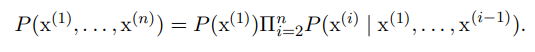
\includegraphics[]{images/joint-prob.png}
\end{center}
This observation is known as the chain rule or \textbf{product rule} of probability.\newline\newline
Two random variables $a$ and $b$ are conditionally independent given a random
variable $c$ if the conditional probability distribution over $a$ and $b$ factorizes in this way for every value of $c$:
\[P(a | b, c) = P(a | c)\]
Equivalently, conditional independence may be stated as:
\[P(a, b | c) = p(a|c)p(b|c)\]
\begin{center}
    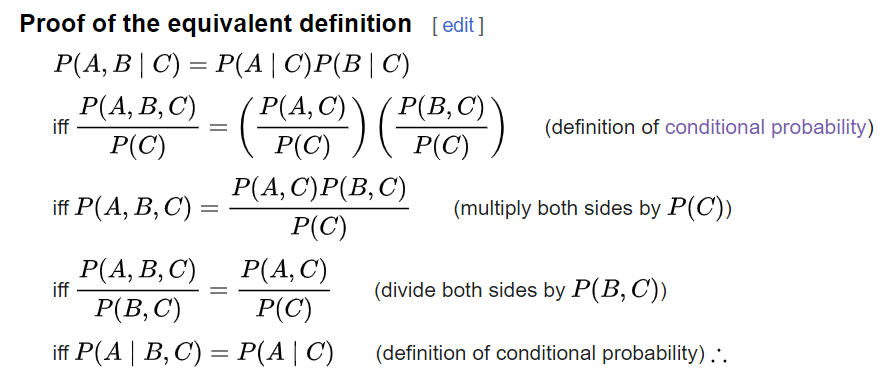
\includegraphics[scale=0.6]{images/proof cond prob.png}
\end{center}


\section{Structured Probabilistic Models}
Deep learning draws upon many modeling formalisms that researchers can use to guide their design efforts and describe their algorithms. One of these formalisms is the idea of structured probabilistic models.\newline\newline
Machine learning algorithms often involve probability distributions over a very large number of random variables. Often, these probability distributions involve \textbf{direct interactions between relatively few variables}. Therefore, Using a single function to describe the entire joint probability distribution can be very inefficient (both computationally and statistically).\newline\newline
Modeling a rich distribution over thousands or millions of random variables is a challenging task, both computationally and statistically. Suppose we only wanted to model binary variables. This is the simplest possible case, and yet already it seems overwhelming. For a small $32 \times 32$ pixel color (RGB) image, there are $2^{3072}$ possible binary images of this form.\newline\newline
In general, if we wish to model a distribution over a random vector $\textbf{x}$ containing $n$ discrete variables capable of taking on $k$ values each, then the naive approach of representing $P(\textbf{x})$ by storing a lookup table with one probability value per possible outcome requires $k^n$ parameters!\newline\newline
This tabular approach is Infeasible for several reasons:
\begin{itemize}
    \item Memory: the cost of storing the representation is too high;

    \item Runtime: inference and sampling are too slow;

    \item Statistical efficiency: As the number of parameters in a model increases, so does the amount of training data needed to choose the values of those parameters using a statistical estimator.
\end{itemize}
Instead of using a single function to represent a probability distribution, we can split a probability distribution into many factors that we multiply together. For example, suppose we have three random variables: $a$, $b$ and $c$. Suppose that $a$ influences the value of $b$ and $b$ influences the value of $c$, but that $a$ and $c$ are independent given $b$. We can represent the probability distribution over all three variables as a product of probability distributions over two variables:
\[p(a, b, c) = p(a)p(b | a)p(c | b)\]
We can greatly reduce the cost of representing a distribution if we are able to find a factorization into distributions over fewer variables. We can describe these kinds of factorizations using graphs. Because the structure of the model is defined by a graph, these models are often also referred to as \textbf{graphical models}.\newline\newline
Tasks for structured probabilistic models:
\begin{itemize}
    \item Density estimation
    \item Denoising
    \item Sample generation
    \item Missing value imputation
    \item Sampling
\end{itemize}


\section{Graphical Models}
Structured probabilistic models provide a formal framework for modeling interactions between random variables. Graphical models use graphs to represent these interactions. Each node represents a random variable. Each edge represents a direct interaction. Paths represent indirect interactions.\newline\newline
Graphical models can be largely divided into two categories: models based on \textbf{directed acyclic graphs}, and models based on \textbf{undirected graphs}.

\subsection{Directed Models}
One kind of structured probabilistic model is the directed graphical model, also known as \textbf{Bayesian Networks}. Directed graphical models are called “directed” because their edges are directed, that is, they point from one vertex to another. The direction of the arrow indicates which variable’s probability distribution is defined in terms of the other’s. Basically, drawing an arrow from
$a$ to $b$ means that the distribution over $b$ depends on the value of $a$. Directed models work best when influence clearly flows in one direction (causal relation).\newline\newline
Given a vector of $n$ random variables $\textbf{x}$, The probability distribution over $\textbf{x}$ is given by:
\[P(x_1, ..., x_n) = \prod_{i=1}^n P(x_i | pa_G(x_i))\]
where $pa_G(x_i)$ represents the parents of $x_i$ in the graph.\newline\newline
For example, the following graph:
\begin{center}
    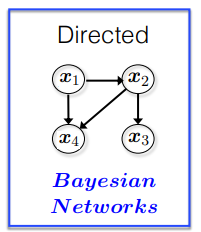
\includegraphics[]{images/directed graph.png}
\end{center}
Corresponds to the following factorization:
\[P(x_1, x_2, x_3, x_4) = P(x_4|x_1, x_2)P(x_3|x_2)P(x_2|x_1)P(x_1)\]
$x_3$ is conditional independent from $x_1$, given $x_2$, while $x_4$ is conditional independent from $x_3$, given $x_1, x_2$.
\begin{center}
    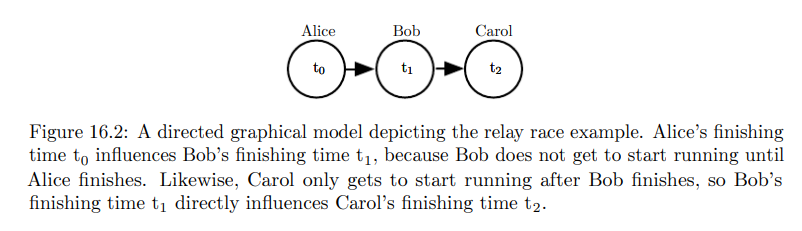
\includegraphics[scale=0.8]{images/relay race.png}
\end{center}
Directed models can drastically reduce the cost of representing a distribution. Let's consider the following example:\newline\newline
Let $t_0, t_1, t_2$ be discrete variables each with 100 possible values. If we want to represent $P(t_0, t_1, t_2)$ with a table, it would need to store 999,999 values ($100^3 - 1$, since the probability of one of the configurations is made redundant by the constraint that the sum of the probabilities be 1). Now we make the \textbf{assumption} that $t_2$ is conditionally independent from $t_0$, given $t_1$:
\[P(t_0, t_1, t_2) = P(t_0)P(t_1 | t_0)P(t_2 | t_1)\]
We can only make a table for each of the conditional probability distributions, then the distribution over $t_0$ requires 99 values, the table defining $t_1$ given $t_0$ requires 9900 values, and so does the table defining $t_2$ given $t_1$. This comes to a total of 19,899 values. This means that using the directed graphical model reduced our number of parameters by a factor of more than 50!\newline\newline
In general, the number of values required to represent a distribution over a variable $x$ is given by:
\[(k - 1) * \prod_{x_p \in pa_{G}}k_{xp}\]
where $k$ is the number of values that $x$ can take, and $k_{xp}$ is the number of values that the parent $x_p$ of $x$ can take.\newline\newline
Basically, the greater the \textbf{degree of dependence} of the graph, the more values are required to represent the distribution.
\begin{center}
    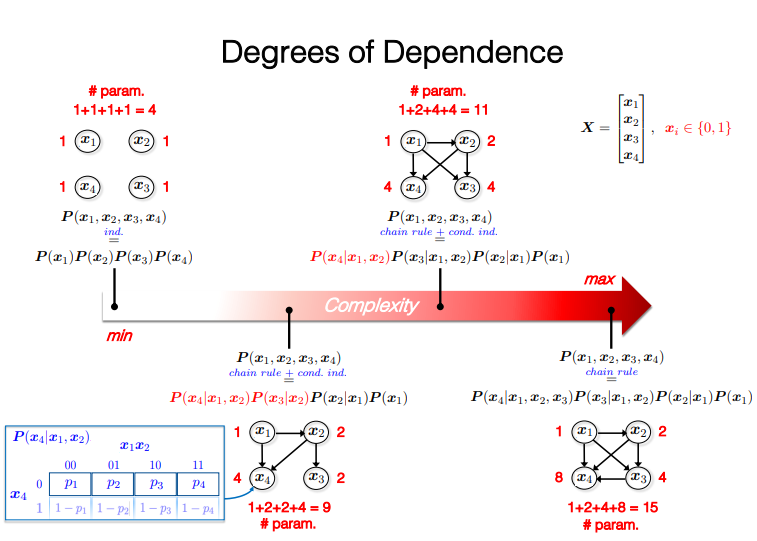
\includegraphics[scale=0.8]{images/degree of dependence.png}
\end{center}
It is important to realize what kinds of information can and cannot be encoded in the graph. The graph, in this case, encodes only simplifying assumptions about which variables are conditionally independent from each other, but it is also possible to make other kinds of simplifying assumptions.

\subsection{Undirected Models}
\textbf{Undirected models} are used when the influence between variables has no clear direction or is best modeled as flowing in both directions.\newline\newline
As an example of such a situation, suppose we want to model a distribution over three binary variables: whether or not you are sick, whether or not your coworker is sick, and whether or not your roommate is sick. Assuming that your coworker and your roommate do not know each other, it is very unlikely that one of them will give the other an infection such as a cold directly. However, it is reasonably likely that either of them could give you a cold, and that you could pass it on to the other. We can model the indirect transmission of a cold with the following undirected graph:
\begin{center}
    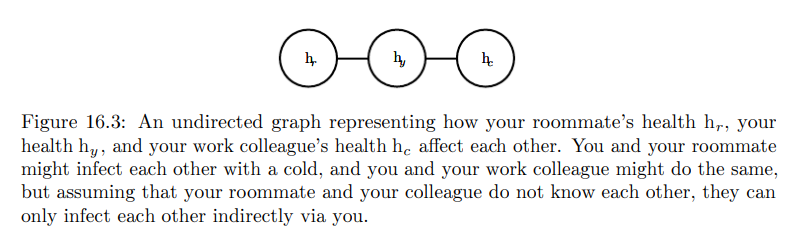
\includegraphics[scale=0.8]{images/undirected models.png}
\end{center}
In this case, there is not a clean, uni-directional narrative on which to base the model.\newline\newline
Formally, an undirected graphical model is a structured probabilistic model defined on an undirected graph $G$. For each clique $C$ in the graph, a factor $\phi(C)$ (also called \textbf{clique potential})  measures the affinity of the variables in that clique for being in each of their possible joint states. The factors are constrained to be
non-negative.\newline\newline
Then, given a vector of random variables $\textbf{x}$, the \textbf{unnormalized probability distribution} over $\textbf{x}$ is given by:
\[\Tilde{P}(\textbf{x}) = \prod_{C \in G}\phi(C)\]
While the unnormalized probability distribution is guaranteed to be non-negative everywhere, it is not guaranteed to sum or integrate to 1. To obtain a valid probability distribution, we must use the corresponding normalized probability distribution:
\[P(\textbf{x}) = \frac{1}{Z}\Tilde{P}(\textbf{x})\]
where the \textbf{partition function} $Z$ is the value that results in the probability distribution summing or integrating to 1. Since $Z$ is an integral or sum over all possible joint assignments of the state $\textbf{x}$
it is often intractable to compute. Due to the intractability of computing $Z$ exactly, we must resort to approximations.

\subsubsection{Energy-Based Models}
A special case of undirected probabilistic models are \textbf{Energy-Based Models}. They enforce $\phi(C) > 0$ by defining the unnormalized probability distribution as:
\[\Tilde{P}(\textbf{x}) = exp(-E(\textbf{x}))\]
\begin{center}
    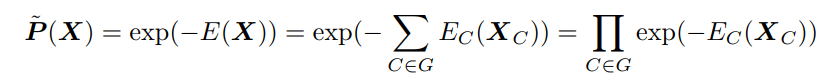
\includegraphics[scale=0.7]{images/undirected2.png}
\end{center}
where $E(\textbf{x})$ is known as the \textbf{energy function} that has to be learned.\newline\newline
Because $exp(z)$ is positive for all $z$, this guarantees that no energy function will result in a probability of zero for any state $\textbf{x}$.\newline\newline
Any distribution of this form is an example of a \textbf{Boltzmann distribution}. For this reason, many energy-based models are called
\textbf{Boltzmann machines}.

\subsubsection{Factor Graphs}
Factor graphs are another way of drawing undirected models that resolve an
ambiguity about graph clique factorization. For example, a clique containing three nodes may correspond to a factor over all three nodes, or may correspond to three factors that each contain only a pair of the nodes.\newline\newline
Factor graphs resolve this ambiguity by explicitly representing the scope of each $\phi$ function.
\begin{center}
    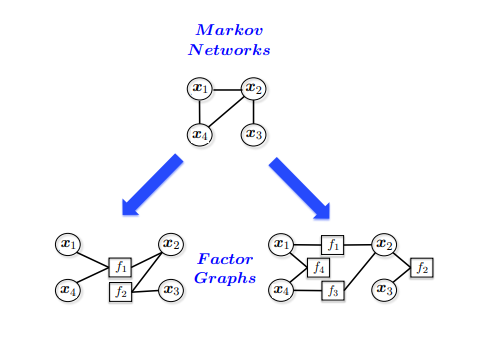
\includegraphics[]{images/factor graphs.png}
\end{center}

\section{Sampling}
If we are able to represent a probability distribution using graphical models, then we can answer any \textbf{probabilistic query}. However, exact inference in graphical models is computational inefficient most of the times. Therefore, we can use sampling for approximate inference. The basic idea is to draw $N$ samples from a sampling distribution $S$ and compute an approximate posterior probability $\hat{\textbf{P}}$. Then, we expect $\hat{\textbf{P}}$ and the true probability $\textbf{P}$ to converge as $N$ increases.\\\\
One advantage of \textit{directed} graphical models is that a simple and efficient procedure called \textbf{ancestral sampling} can produce a sample from the joint distribution represented by the model.\newline\newline
The basic idea is to sort the variables $x_i$ in the graph into a topological ordering (i.e. from the variables with fewer parents), and sample each node given its parents. In other words, we first sample $x_1 \sim P(x_1)$, the sample $x_2 \sim P(x_2|pa_G(x_2))$, and so on, until we finally sample $x_n \sim P(x_n|pa_G(x_n))$.\newline\newline
So long as each conditional distribution $P(x_i | pa_G(x_i))$ is easy to sample from, then the whole model is easy to sample from. Without the topological sorting, we might attempt to sample a variable before its parents are available.\newline\newline
One drawback of ancestral sampling is that it does not support every conditional sampling operation. When we wish to sample from a subset of the variables in a directed graphical model, given some other variables, we often require that all the conditioning variables come earlier than the variables to be sampled in the ordered graph. Unfortunately, ancestral sampling is applicable only to directed models.\newline\newline
Sampling from an \textbf{undirected model} seems to require resolving cyclical dependencies. Every variable interacts with every other variable, so there is no clear beginning point for the sampling process. Unfortunately, drawing samples from an undirected graphical model is an expensive, multi-pass process. The conceptually simplest approach is \textbf{Gibbs sampling}.

